\scanpage{62}
correspondant, sur la sphère standard, à la région ci-contre, délimitée par le contour
\[
P_+Q_1R_0^-\unsure{S_0^+|D_0^+}R_0^+S_0^-P_-Q_\infty R_1^-S_1^+P_+
\]
\figure{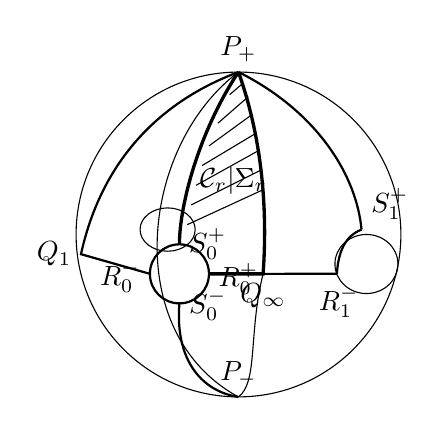
\begin{tikzpicture}[scale=1.25,>=stealth]
\coordinate(N)at(0,1.65);\coordinate(S)at(0,-1.65);\coordinate(L)at(-1.6,-.2);\coordinate(Q)at(.25,-.4);
\draw[thin](0,0)circle(1.65);
\draw[thin](N)..controls(-1,.9)and(-1.2,-1)..(S);
\draw[thick](N)..controls(-1.2,1.2)and(-1.5,.25)..(L)--(-.9,-.4);
\draw[very thick](N)..controls(-.4,1.05)and(-.6,.3)..(-.6,-.1);
\draw[very thick](N)..controls(.23,1)and(.3,.3)..(Q)--(-.3,-.4);
\draw[thick](Q)--(1,-.4);\draw[thick](N)..controls(.8,1.25)and(1.2,.6)..(1.25,.05);
\draw[thick](-.6,-.4)circle(.3);\draw[thin](1.3,-.3)ellipse(.32 and .3);
\draw[thick](1,-.4)..controls(1.02,-.05)and(1.18,.02)..(1.25,.05);
\draw[thin](-.72,.05)ellipse(.28 and .22);
\draw[thick](-.6,-.7)..controls(-.65,-1.3)and(-.35,-1.6)..(S);
\draw[thin](Q)..controls(.1,-1)and(.2,-1.5)..(S);
\foreach \a/\b/\c/\d in {-.52/.1/.24/.45,-.48/.3/.22/.65,-.43/.5/.2/.85,-.37/.7/.18/1.03,-.3/.9/.14/1.22,-.21/1.13/.1/1.4,-.09/1.42/.05/1.54}{\draw[thin](\a,\b)--(\c,\d);}
\node[above]at(N){$P_+$};\node[above]at(S){$P_-$};\node[left]at(L){$Q_1$};\node[below]at(Q){$Q_\infty$};
\node[left]at(-.9,-.43){$R_0^-$};\node[right]at(-.3,-.45){$R_0^+$};\node[right]at(-.6,-.1){$S_0^+$};\node[right]at(-.6,-.72){$S_0^-$};
\node[below]at(1.02,-.43){$R_1^-$};\node[above right]at(1.25,.05){$S_1^+$};
\node at(-.05,.55){$\unsure{\mathcal C_r|\Sigma_r}$};
\end{tikzpicture}}
Les régions $\widetilde\Sigma_r$ sont permutées de façon simplement transitive par $\Gamma=\mathcal G_J\times(1,\tau)$. Elles sont simplement connexes, et permettent donc de définir des
\[
\deleted{(42)}\qquad\Pi_r=\Pi_i^{\omega\varepsilon}=\Pi_1(\widetilde\Sigma;\widetilde\Sigma_r)=\Pi_1(\Sigma^*;\Sigma_r^*)
\]
\deleted{et des isom} \deleted{qui} mais qui sont reliés par un syst. transitif d'iso. à l'aide du gr. de $\Gamma$, de sorte qu'on peut identifier tous ces groupes entre eux. En fait, on trouve des isom. d'épinglage
\[
(42)\qquad\Psi_r:\Pi_{0,3}\longrightarrow\Pi_r=\unsure{\Pi_i|\Pi}^{\omega,\unsure{i|\varepsilon}}=\Pi_1(\widetilde\Sigma;\widetilde\Sigma_r)
\]
($\psi_r$ majuscule

\deleted{en identifiant}
en composant
\diagram{\begin{tikzcd}[ampersand replacement=\&,column sep=large]
\Pi_{03}\arrow[r,shorten >=1.7em]\arrow[r,"\psi_r=\psi_\varepsilon^{\omega,i}"]\&\begin{array}{c}\Pi_1(\widetilde\Sigma,P_\varepsilon)\\\simeq\Pi_1(\Sigma^*,P_\varepsilon)\end{array}\arrow[r,leftrightarrow,"\varphi_r^{-1}"]\&\Pi_r
\end{tikzcd}}
où \deleted{$\unsure{\varphi}$}
\[
\varphi_r:\Pi_r\longrightarrow\Pi_\varepsilon=\Pi_1(\widetilde\Sigma,P_\varepsilon)
\]
est l'``isomorphisme de transition'' correspondant à la région $1$-connexe $\Sigma_r$, et au point $P_\varepsilon$ de $\Sigma_r$.
\margin{61}
